%mark = star, diamond, square, otimes
%\documentclass{article}
%\usepackage{pgfplots}
%\usepackage[justification=centering]{caption}
%\pgfplotsset{compat=newest}
%\begin{document}
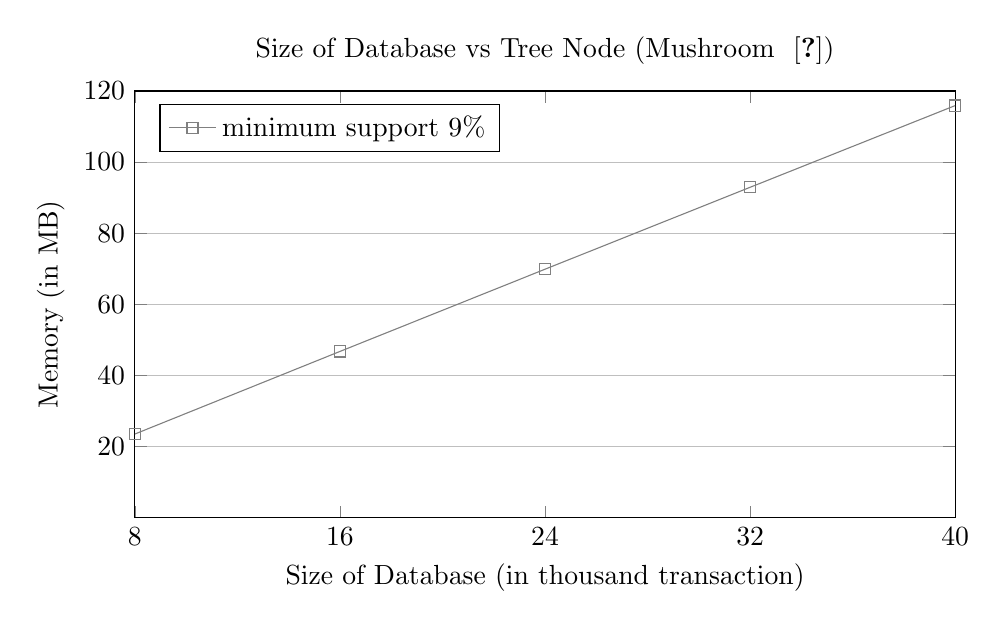
\begin{tikzpicture}
\begin{axis}[
	title={Size of Database vs Tree Node (Mushroom ~\cite{dataset})},
	width=12cm,
	height=7cm,
    xlabel={Size of Database (in thousand transaction)},
    ylabel={Memory (in MB)},
    xmin=8, xmax=40,
    ymin=0, ymax=120,
    xtick={8,16,24,32,40},
    ytick={20,40,60,80,100,120},
    legend pos=north west,
    ymajorgrids=true,
    grid style={line width=.2pt,draw=gray!50},
]
 
\addplot[
    solid,color=gray, every mark/.append style={solid, fill=gray}, mark=square
    ]
    coordinates {
			(8, 23.504)
			(16,46.736)
			(24,69.861)
			(32,92.903)
			(40,115.888)



	};
    \addlegendentry{minimum support 9\%}

\end{axis}
\end{tikzpicture}
%\end{document}